\chapter{Method}

This chapter will present the two landmark detector methods and their inner workings. In addition, a novel quality indicator for SSS data is presented.

\section{Quality Indicator for Side Scan Sonar Data}

The novel quality indicator calculates the overlapping of consecutive swaths, considering the ground range at maximum sensor opening. The motivation behind the quality indicator is to easily be able to pick out the areas of a sonar image where the turning of the AUV has affected the quality of the data, and anomalies and garbage data are expected. \cref{fig:r_eff} shows the SSS configuration, where $\theta$ is the mounting angle for the transducers from the horizontal line, $\alpha$ is the sensor opening, $h$ is the AUVs altitude above the seafloor, and $r_{g, max}$ is the maximum ground range. Because of varying altitudes, $h$, the maximum sonar ground range does not represent the range where we expect to find meaningful data. The effective ground range on the other side, $r_{g, eff}$, is a better representation and is given by:

\begin{equation}
    r_{g,eff} = \frac{h}{tan(\theta - \frac{\alpha}{2})}
    \label{eq:r_g_eff}
\end{equation}

\begin{figure}
    \centering
    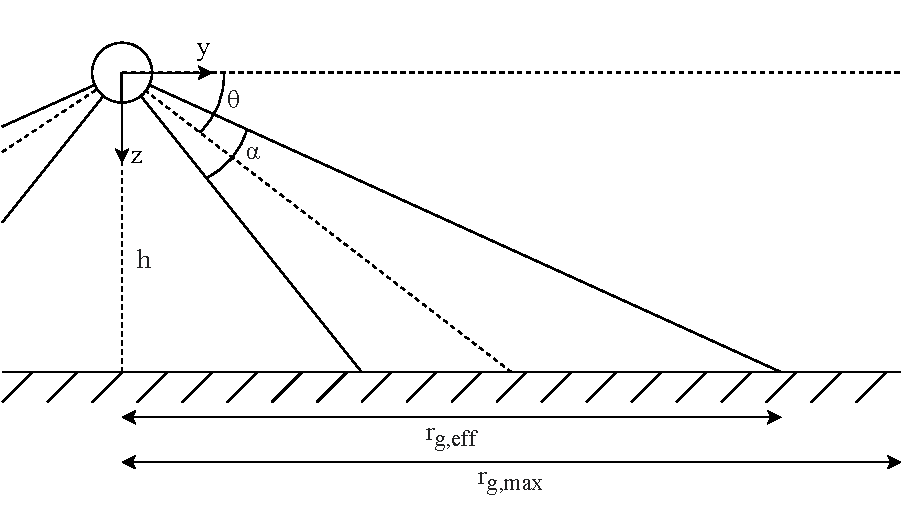
\includegraphics[width=0.8\textwidth]{figures/r_eff.drawio.pdf}
    \caption{Side scan sonar where $r_{eff}$, used in calculating the quality indicator, is shown.}
    \label{fig:r_eff}
\end{figure}

\cref{fig:quality_ind} show the AUV at two consecutive timesteps, where $\Delta \psi$ is the absolute change in heading between the two timesteps (positive for both left and right turn), $\Delta d$ the distance traveled in the xy-plane between the two timesteps. $r_{g, max}$, $r_{g, eff}$ still the maximum and effective ground range, respectivley. $l$ is the distance between the AUV and the point on the swath where the next swath is crossing (could be at infinity in case of $\Delta \psi = 0$) and is given by:

\begin{equation}
    l = \frac{\Delta d}{tan(\Delta \psi)}
    \label{eq:l_qi}
\end{equation}

Using the above results, the following quality indicator is proposed:

\begin{equation}
    q = \frac{1}{2}(tanh( \,k\, (\frac{l}{r_{g, eff}} - \frac{1}{2})) + 1)
\end{equation}

where $k$ is a tuning parameter used to tune the sensitivity of the quality indicator. 

\begin{figure}
    \centering
    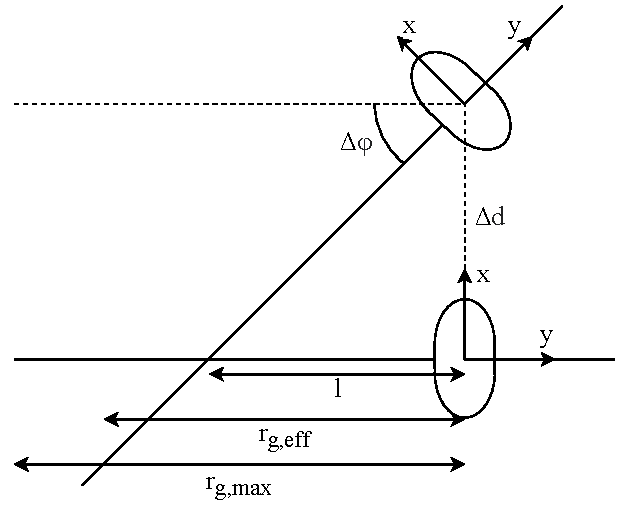
\includegraphics[width=0.55\textwidth]{figures/quality_ind.drawio.pdf}
    \caption{The figure shows an AUV for two consecutive timestamps, showing how the swaths can overlap due to the AUV turning.}
    \label{fig:quality_ind}
\end{figure}

\section{1D Landmark Detector using Peak Detection}

The 1D landmark detector, as in \cite{Al-Rawi2017LandmarkImages,} does peak detection in scan lines to find shadows and echoes and filter out non-significant echoes and shadows using a simple threshold. In this context, peak detection finds all local maxima in the swath. Landmarks are detected in one swath at a time, and peak detection is performed separately for the left and right parts of the swath. The first step for detecting meaningful peaks is to perform a smoothing of the swath, which is done by using a cubic spline. Next, the echoes are detected by detecting all peaks in the swath, and the shadows are detected by flipping the swath and detecting all peaks in the flipped signal. In addition to the position of all the peaks, the prominence and the width half-prominence are found. \cref{fig:1D_swath_w_landmarks} shows the result of detecting the echoes and shadows using peak detection. In addition, the peak of the FBR to the left swath is shown with its prominence and half-prominence width.
Further, all the shadows and echoes are filtered to detect landmarks. The first step is to remove the echo from the FBR and the shadow from the blind zone, as these are not generated from a landmark. These are the two most significant echoes and shadows in \cref{fig:1D_swath_w_landmarks}. Next, all echoes and shadows are filtered by a simple threshold given by:

\begin{equation}
    E = \frac{2\times width}{prominence}
    \label{eq:1D_thres}
\end{equation}

\begin{figure}
    \centering
    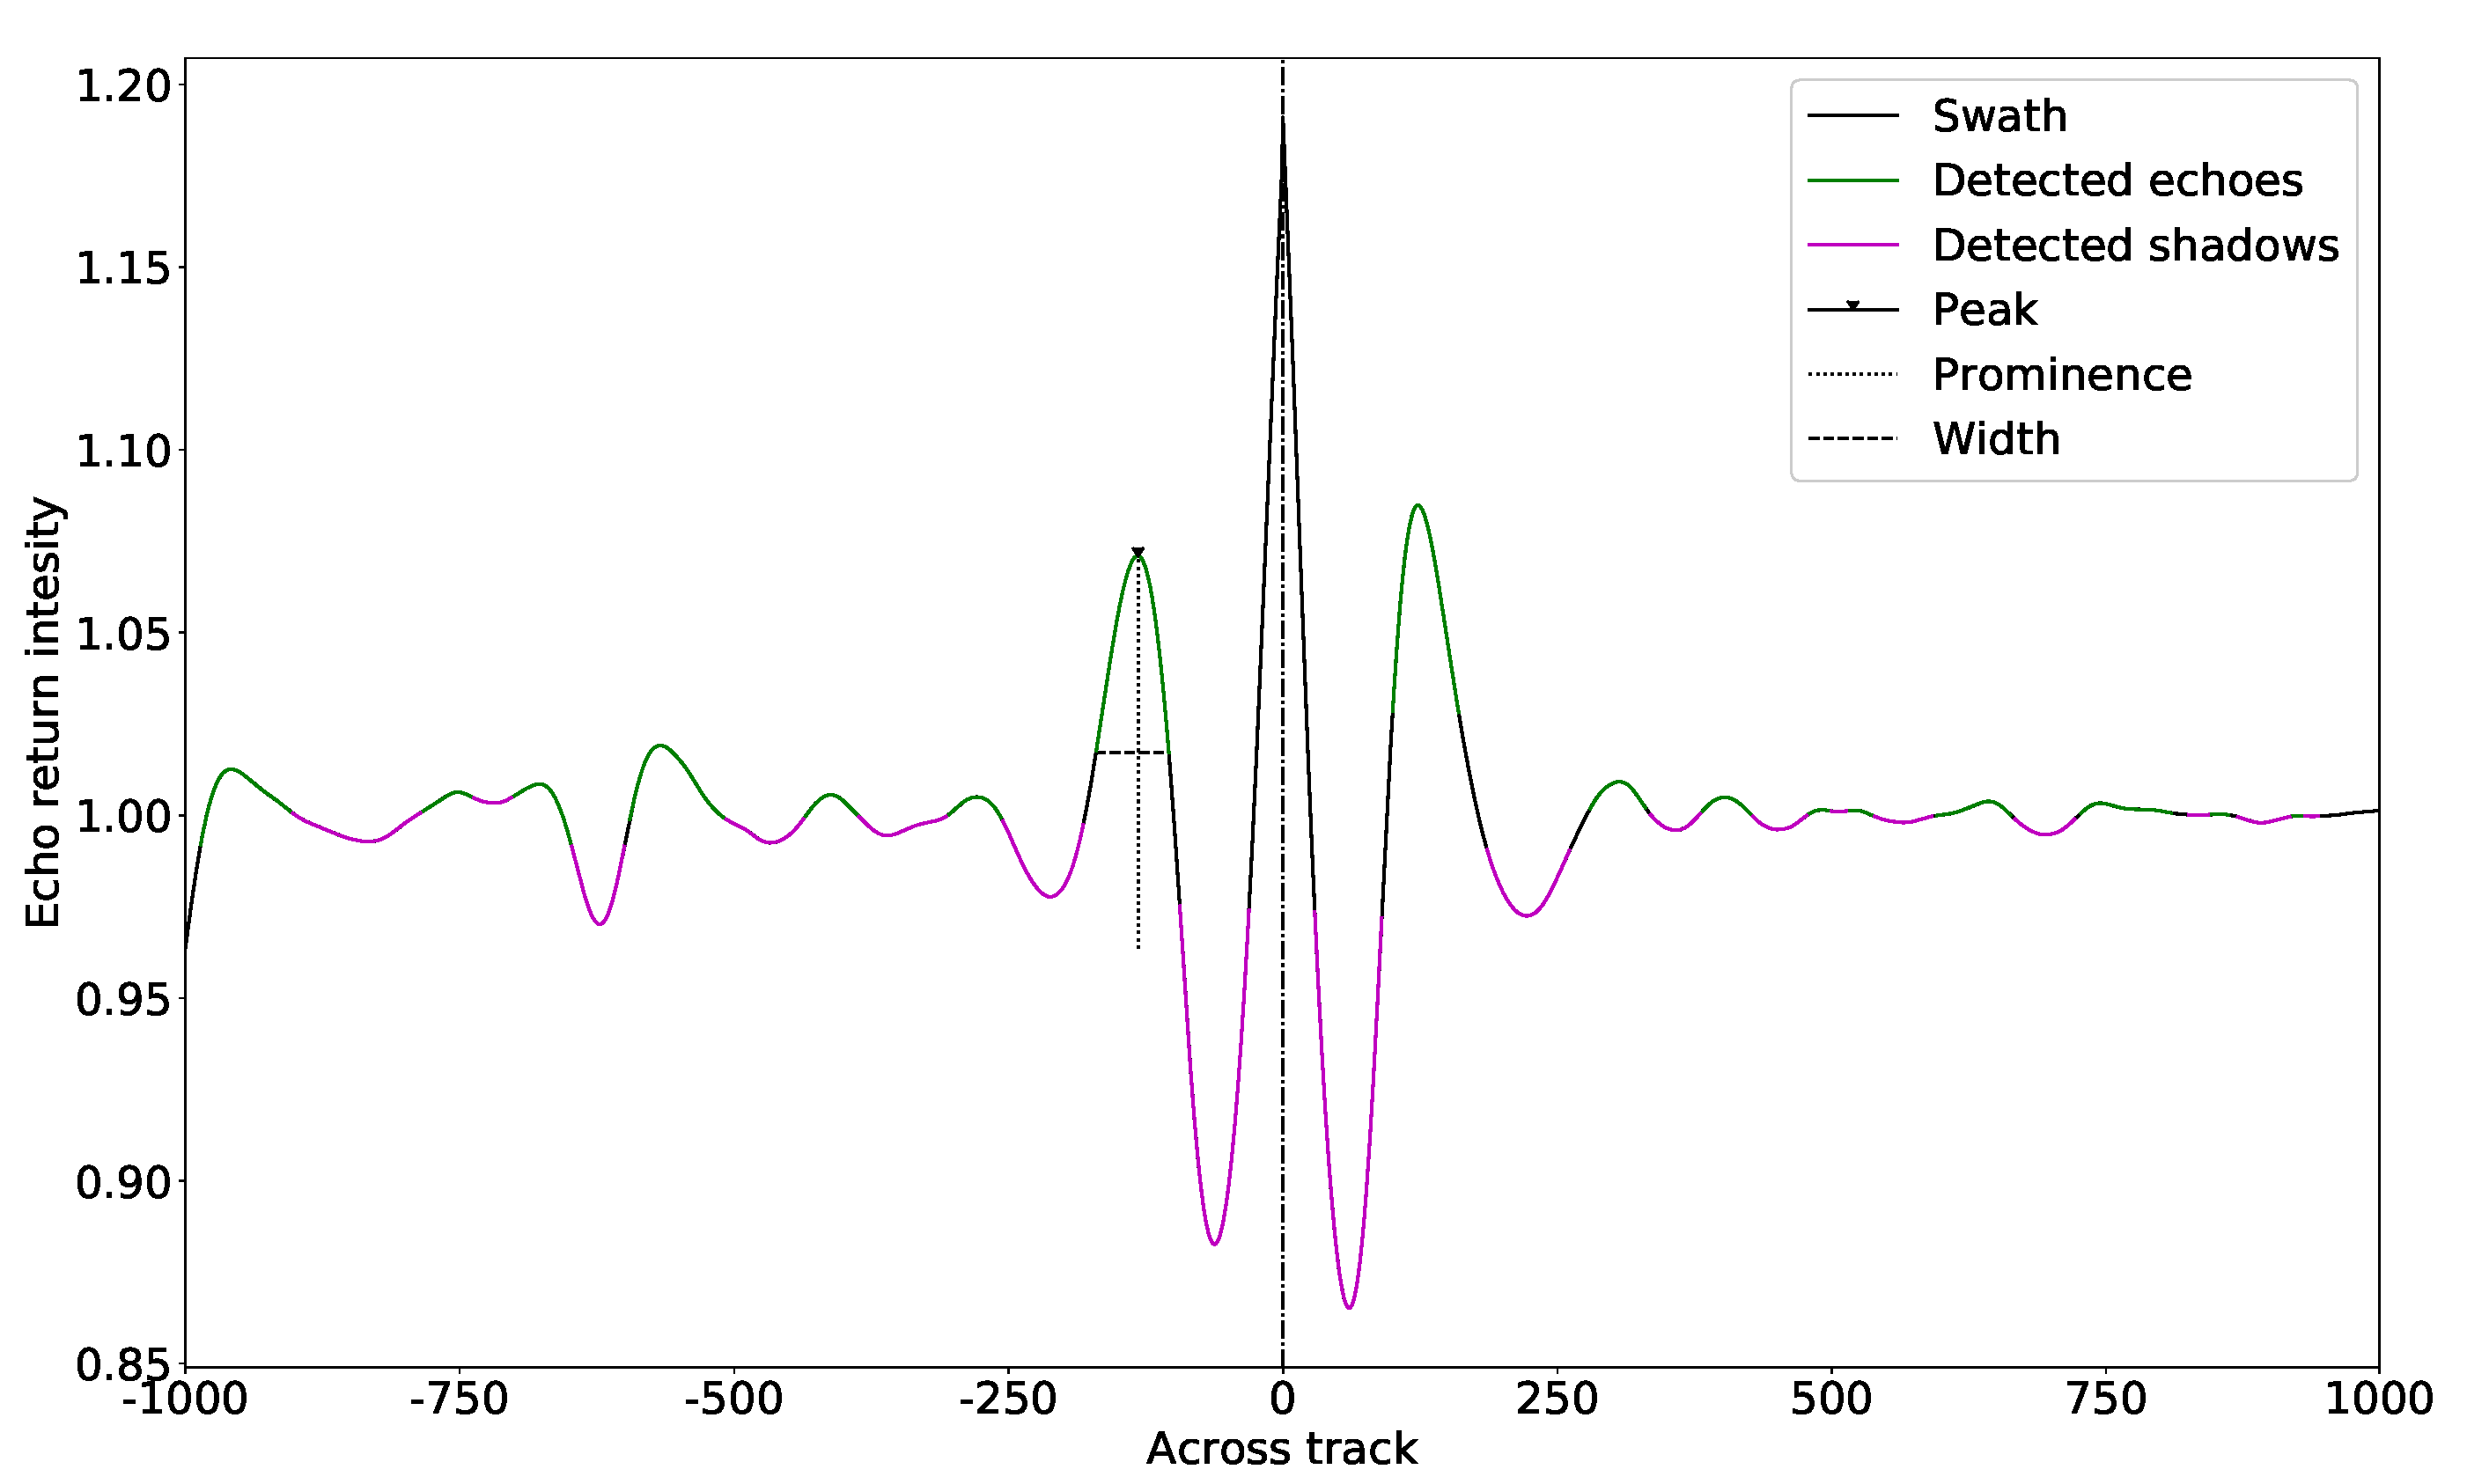
\includegraphics[width=0.8\textwidth]{figures/1D_swath_w_landmarks.eps}
    \caption{Normalized swath with all detected echoes and landmarks before filtering. The peak at the first bottom return for the left swath with its prominence and half-prominence width is also shown.}
    \label{fig:1D_swath_w_landmarks}
\end{figure}

In \cite{Al-Rawi2017LandmarkImages}, un-normalized SSS data is used, but the use of normalized data is suggested as an improvement. This report will present the result of performing landmark detection on normalized and unnormalized data. In addition, further improvements are suggested by applying morphological operators to remove thin landmarks and improve consistency. In the works of this report, a combination of a closing operation followed by a closing operation is performed. 2D binary images are constructed for shadows and echoes to perform morphological operations.  

\section{2D Landmark Detector using Expert Rules}

The 2D landmark detector, as in \cite{Leblond2019SonarProject}, finds shadows by intensity thresholding and uses a set of rules to filter out the shadows of the right size and form. The first step is to perform an intensity thresholding on all the pixels to find shadows. The suggested intensity threshold is:

\begin{equation}
    t_i = \frac{\Bar{I(x,y)}}{2}
    \label{eq:orginal_int_thres}
\end{equation}

where $\Bar{I(x,y)}$ is the average pixel intensity in the sonar image. However, this threshold produced close to no shadows from the data, so a new intensity threshold is suggested:

\begin{equation}
    t_i = (\Bar{I(x,y)} - I(x,y)_{min}) k_i + I(x,y)_{min} 
\end{equation}

where $I(x,y)_{min}$ is the average over the $100$ smallest pixels, which is done to be more robust against outliers in the data. $k_i$ is a tuning parameter ranging from $0$ to $1$. Using the result from the intensity thresholding, a series of filtering rules are applied to filter out shadows. First, the shadows get filtered based on how many swaths they span over, where both minimum and maximum height filtering is applied. Secondly, filtering based on the area of the shadows in $pixels^2$ is applied. To account for how the grazing angle affects the shadows, the area is corrected by

\begin{equation}
    A_{corr} = A_s \times r = A \times \frac{r_{ob,min}}{r_{ob}}
    \label{eq:corrected_area}
\end{equation}

where $r_{ob, min}$ is a reference object ground range that is tuneable, $r_ob$ is the ground range to the object, and $A_s$ is the area of the shadow in $pixels^2$. The last step is to filter the shadows based on how much of the bounding box that surrounds them that are filled, where the fraction of filled is given by

\begin{equation}
    \frac{A_s}{A_{bb}}
    \label{eq:fill_rate_bb}
\end{equation}

where $A_{bb}$ is the area of the bounding box surrounding the shadow. The bounding box's fill rate is compared to the fill rate threshold, $t_{fr}$. In addition to the proposed rules and tuning parameters, this report adds a gaussian blurring of the sonar image and a closing operation to generate consistent landmarks. The structuring elements (SE) are both restricted to be quadratic, giving two new tuning parameters, $k_g$ and $k_c$, for the size of the quadratic gaussian structuring element and the quadratic structuring element used for the closing operation, respectively. \cref{tab:2D_tuning_rules} summarises all tunable parameters and corresponding filtering rules. 

\begin{table}
    \begin{center}
    \begin{tabular}{|l|l|}
    \hline
        \textbf{Tunable parameter} & \textbf{Filtering rule}                            \\ \hline
        $k_g$             & Gaussian blurring of the sonar image with SE of size $k_g$  \\ \hline
        $k_i$             & $I(x,y) < (\Bar{I(x,y)} - I(x,y)_{min}) k_i + I(x,y)_{min}$ \\ \hline
        $k_c$             & Morphological closing on the shadows with SE of size $k_c$  \\ \hline
        $n_{swaths,min}$  & $n_{swaths} > n_{swaths,min}$                               \\ \hline
        $n_{swaths,max}$  & $n_{swaths} < n_{swaths,max}$                               \\ \hline
        $r_{ob,min}$      & $A_{corr} = A_s \times \frac{r_{ob,min}}{r_{ob}}$           \\ \hline
        $A_{min}$         & $A_{corr} > A_{min}$                                        \\ \hline
        $t_{fr}$          & $\frac{A_s}{A_{bb}} > t_{fr}$                               \\ \hline
    \end{tabular}
    \end{center}
    \caption{The table shows all the tunable parameters for the 2D landmark detector and the corresponding filtering rules applied.}
    \label{tab:2D_tuning_rules}
\end{table}

\section{Qualitative comparison}

This report makes a qualitative comparison of the landmark detectors' results to compare them against each other. To make a meaningful comparison, some grounds for comparison must be set. First and foremost, an understanding of what part of a sonar image is considered a landmark and what is just considered background. Next, an understanding of what makes up consistent landmarks is also essential. Lastly, some grounds for comparing the tuning process have to be defined. 

To compare the methods, an understanding of what parts of the sonar image are actual landmarks and what properties are consistent with a landmark. Firstly, a division into echo and shadow landmarks has to be done. Echoes are typically generated by objects standing out from the seafloor, reflecting more sound and generating a more significant echo intensity in the sonar image. On the other hand, shadows are generated by occlusion, either by objects on the seafloor or simply by holes at the seafloor, and give dark areas in the sonar image. Whenever an echo landmark is detected, it is also expected to detect a shadow landmark. This is because the object generating the increased echo is expected to occlude some parts of the ultrasonic pulse and generate a shadow. 

Landmark consistency is an essential qualitative measure and tells to what extent a landmark detection method can detect a landmark as one coherent landmark or several minor landmarks. The opposite is when what appears as one consistent landmark in the sonar image is either only detected partially or as several minor landmarks. The problem with partially detected or split landmarks is that small changes in how the landmark is observed can result in a landmark with a widely different form or size being detected. Further, this will lead to problems for the data association. 

Another vital measure when comparing landmark detection methods is how sensitive, complex, and intuitive the detector tuning is. Sensitivity is vital because if a method has a significant sensitivity, small changes in the operating conditions can significantly change performance. On the other hand, if the method has an acceptable performance over a wide range of parameters, it is more likely that the same is evident over a wide range of operating conditions. Next, the complexity of the tuning says something about how difficult it is to obtain good results and how interconnected the different parameters are in each other. Suppose the parameters do not have a great deal of interconnection. In that case, it is possible to tune one parameter at a time sequentially and end up with acceptable performance. In the opposite case, tuning one parameter will significantly influence the other parameters' effect on the performance, making it more difficult to obtain acceptable performance. Hence, the tuning is more complex. Last, how intuitive a tuning process is, is tightly related to the meaning of the tuning parameters. If the parameters are only arbitrary sizes, how they affect the tuning process is not intuitive. On the other hand, the tuning can be said to be more intuitive if there is a direct relation between the parameters and the effect they have on the performance.     
